\documentclass[../main.tex]{subfiles}
\graphicspath{{\subfix{../images/}}}
\begin{document}
\hypertarget{parametricintegrationanswers}{\subsection*{Answers - Parametric integration (\hyperlink{parametricintegrationlink}{page \pageref{parametric integration}})}}

\label{Parametric integration answers}

\begin{enumerate}
\begin{spacing}{1.5}
    \item 
    Evaluate $\int_0^1 y\,dx$ for the parametric curve given by $\begin{cases} x=4-t \\ y=t^2-3t \end{cases}$

    Write $dx$ in terms of $t$ and $dt$

    $dx=-dt$

    Calculate the bounds in terms of $t$:

    Upper: $1=4-t \Rightarrow t=3$

    Lower: $0=4-t \Rightarrow t=4$

    Rewrite integral in terms of $t$:

    $\int_4^3 (t^2-3t)\,-dt=\int_4^3 (3t-t^2)\,dt$

    Integrate and calculate definite integral:

    $\Bigl[\frac{3t^2}{2}-\frac{t^3}{2}\Bigr]_4^3=\frac{11}{6}$

    \item 
    Write $dx$ in terms of $t$ and $dt$

    $\frac{dx}{dt}=\cos{t}$

    $dx=\cos{t}\,dt$

    Calculate bounds in terms of $t$:

    Upper: $1=\sin{t} \Rightarrow t=\frac{\pi}{2}$

    Lower: $-\frac{1}{2}=\sin{t} \Rightarrow t=-\frac{\pi}{6}$

    Rewrite integral in terms of $t$:

    $\int_{-\frac{\pi}{6}}^{\frac{\pi}{2}}2(\cos{t}-\sin{t})\cos{t}\,dt=2\int_{-\frac{\pi}{6}}^{\frac{\pi}{2}}\cos^2{t}-\sin{t}\,dt$

    Simplify using trig identities:

    $2\int_{-\frac{\pi}{6}}^{\frac{\pi}{2}}\cos{2t}+1-\sin{t}\,dt$

    $=\Bigl[\frac{\sin{2t}}{2}+t+\frac{\cos{2t}}{2}\Bigr]_{-\frac{\pi}{6}}^{\frac{\pi}{2}}=\frac{\sqrt{3}}{4}-\frac{3}{4}+\frac{2\pi}{3}=\frac{3\sqrt{3}-9+8\pi}{12}$

    \item 
    $\frac{dx}{dt}=\sec^2{t}\\
    dx=\sec^2{t}\,dt$

    Calculate bounds in terms of $t$:

    Upper: $\tan{t}=\sqrt{3} \Rightarrow
    t=\frac{\pi}{3}$

    Lower: $\tan{t}=0 \Rightarrow t=0$

    Rewrite the integral in terms of $t$:

    $\int_0^{\frac{\pi}{3}} \sin{t}\sec^2{t}\,dt=\int_0^{\frac{\pi}{3}}\sin{t}\frac{1}{\cos^2{t}}\,dt$

    Integrating:

    $\Bigl[\frac{1}{\cos{t}}\Bigr]_0^{\frac{\pi}{3}}=1$

    \item 
    Work out the area above the $x$-axis, and then multiply by 2.

    In other words:

    $A=2\int_{-r}^{r} y\,dx$

    Find $dx$:

    $\frac{dx}{dt}=r\cos{t}\\
    dx=r\cos{t}\,dt$

    Calculate bounds in terms of $t$:

    Upper: $r=r\cos{t} \Rightarrow 1=\cos{t} \Rightarrow t=0$

    Lower: $-r=r\cos{t} \Rightarrow -1=\cos{t} \Rightarrow t=\pi$

    Rewrite the integral in terms of $t$:

    $\int_{\pi}^0 r\sin{t}\times -r\sin{t}\,dt=-r^2\int_{\pi}^{0}\sin^2{t}\,dt$

    Use the cosine double angle rule to simplify before integrating:

    $-r^2\int_{\pi}^0 \frac{1}{2}-\frac{\cos{2t}}{2}\,dt$

    $-r^2\Bigl[\frac{t}{2}-\frac{\sin{2t}}{4}\Bigr]_{\pi}^{0}$

    $=-r^2\Bigl[\Bigl(0-0\Bigr)-\Bigl(\frac{\pi}{2}-0\Bigr)\Bigr]=-r^2\Bigl[-\frac{\pi}{2}\Bigr]=\frac{\pi r^2}{2}$

    Multiplying by 2 to get the full area of the circle gives $2\times \frac{\pi r^2}{2}=\pi r^2$ as required.

    \item 
    Need to calculate the area above the $x$-axis, then double.
    \begin{figure}[h]
        \centering
        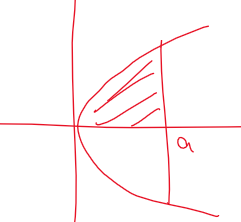
\includegraphics[width=0.15\linewidth]{images/parametricintegration3.png}
    \end{figure}

    Write $dx$ in terms of $t$ and $dt$:

    $\frac{dx}{dt}=2at\\
    dx=2at\,dt$

    Bounds in terms of $t$:

    Upper: $a=at^2 \Rightarrow t=1$

    Lower: $0=at^2 \Rightarrow t=0$

    Rewrite the integral in terms of $t$:

    $\int_0^1 2at\times 2a\,dt=\int_0^1 4a^2t^2\,dt=4a^2\int_0^1 t^2\,dt$

    $=4a^2\Bigl[\frac{t^3}{3}\Bigr]_0^1=\frac{4a^2}{3}$

    Double the result to get the whole area of $\frac{8a^2}{3}$

    \item 
    $\frac{dx}{dt}=-2\sin{2t} \Rightarrow dx=-2\sin{2t}\,dt$

    Write integral in terms of $t$:

    $\int_{-\frac{\pi}{4}}^{\frac{3\pi}{4}} 2(\cos{t}+\sin{t})\times -2\sin{2t}\,dt$

    Using sine double angle rule:

    $\int_{-\frac{\pi}{4}}^{\frac{3\pi}{4}} 2(\cos{t}+\sin{t})\times -4\sin{t}\cos{t}\,dt=-8\int_{-\frac{\pi}{4}}^{\frac{3\pi}{4}} \sin{t}\cos^2{t}+\sin^2{t}\cos{t}\,dt$

    Integrate:

    $-8\Bigl[-\frac{\cos^3{t}}{3}+\frac{\sin^3{t}}{3}\Bigr]_{-\frac{\pi}{4}}^{\frac{3\pi}{4}}$

    Evaluate:

    $\cos{\frac{3\pi}{4}}=-\frac{\sqrt{2}}{2}, \sin{\frac{3\pi}{4}}=\frac{\sqrt{2}}{2}$

    $\cos{-\frac{\pi}{4}}=\frac{\sqrt[root]{2}}{2}, \sin{-\frac{\pi}{4}}=-\frac{\sqrt{2}}{2}$

    $-8\Bigl(\Bigl[-\frac{1}{3}(\frac{\sqrt{2}}{2})^3+\frac{1}{3}(\frac{\sqrt{2}}{2})^3\Bigr]-\Bigl[-\frac{1}{3}(\frac{\sqrt{2}}{2})^3+\frac{1}{3}(-\frac{\sqrt{2}}{2})^3\Bigr]\Bigr)$

    $-8\Bigl[\frac{8\sqrt{2}}{24}\Bigr]=-\frac{8\sqrt{2}}{3}$

    The area must be positive, the bounds would have been in the wrong order, therefore the area is $\frac{8\sqrt{2}}{3}$

    \item 
    We will find the area of the top-right quadrant and then multiply the answer by 4.
    
    Find $dx$ in terms of $t$ and $dt$:

    $\frac{dx}{dt}=-3\cos^2{t}\sin{t} \Rightarrow dx=-3\sin{t}\cos^2{t}\,dt$

    Find the bounds in terms of $t$:

    Upper: $1=\cos^3{t} \Rightarrow t=0$

    Lower: $0=\cos^3{t} \Rightarrow t=\frac{\pi}{2}$

    The total area is now an integral in terms of $t$:

    $4\times\int_{\frac{\pi}{2}}^{0} -3\sin^4{t}\cos^2{t}\,dt$

    Rewriting so we can use the sine double-angle rule:

    $-3\int_{\frac{\pi}{2}}^{0}4\sin^2{t}\cos^2{t}\sin^2{t}\,dt=-3\int_{\frac{\pi}{2}}^{0} \sin^2{2t}\sin^2{t}\,dt$

    Use the cosine double-angle rule:

    $-\frac{3}{2}\int_{\frac{\pi}{2}}^{0} \sin^2{2t}(1-cos{2t})\,dt=-\frac{3}{2}\int_{\frac{\pi}{2}}^{0} \sin^2{2t}-\sin^2{2t}\cos{2t}\,dt$

    Split into two integrals, rewriting the first using the cosine double-angle rule:

    $-\frac{3}{4}\int_{\frac{\pi}{2}}^{0} 1-\cos{4t}\,dt--\frac{3}{2}\int_{\frac{\pi}{2}}^{0} \sin^2{2t}\cos{2t}\,dt$

    Integrate the second integral using a substitution of $u=\sin{2t}$

    $\Bigl[-\frac{3t}{4}+\frac{3\sin{4t}}{16}+\frac{\sin^3{2t}}{6}\Bigr]_{\frac{\pi}{2}}^{0}$

    $=\Bigl(0\Bigr)-\Bigl(-\frac{3\pi}{8}+0+0\Bigr)=\frac{3\pi}{8}$



\end{spacing}  
\end{enumerate}
\end{document}